\documentclass[twocolumn]{article}
\usepackage{xeCJK} % 支持中文
\usepackage[left=2cm,right=2cm,top=2cm,bottom=2cm]{geometry} % 设置页边距
\usepackage{abstract} % 定制摘要

\usepackage{indentfirst} % 设置首行缩进

% 原模板使用 SimSun/SimHei；macOS 无此二字体，改用系统自带宋体/黑体
\setCJKmainfont{Songti SC}[BoldFont = Heiti SC]
\setCJKsansfont{Heiti SC}
\setmainfont{Times New Roman} % 设置英文字体


% =================================
% 数学与公式
% =================================
\usepackage{amsmath}        % AMS 提供的数学公式增强宏包，提供 align, gather 等环境
\usepackage{amssymb}        % 包含大量数学符号，如 R（实数集）、\lesssim 等
\usepackage{amsfonts}       % AMS 提供的数学字体，用于特殊字体（如花体字母）
\usepackage{bm}             % 使公式中的粗体符号（如向量）显示为直立粗体 (\bm)

% =================================
% 图形、表格与浮动体
% =================================
\usepackage{graphicx}       % 引入图片（使用 \includegraphics 命令）
\usepackage{float}          % 增强对浮动体（图、表）的控制，例如 H 定位符
\usepackage{booktabs}       % 绘制专业、美观的三线表（使用 \toprule, \midrule, \bottomrule）
\usepackage{multirow}       % 表格中合并行
\usepackage{makecell}       % 表格中换行和调整单元格边距
\usepackage{caption}        % 更好地自定义图表标题格式
\usepackage{subcaption}     % 在一个浮动体中并排放置多个子图或子表


% =================================
% 链接与排版增强
% =================================
\usepackage{hyperref}       % 生成可点击的超链接（目录、引用、参考文献等），通常应最后加载
\hypersetup{
	colorlinks=true,        % 彩色链接
	linkcolor=black,        % 内部链接颜色
	citecolor=blue,         % 引用链接颜色
	urlcolor=blue           % URL 链接颜色
}
\usepackage{enumerate}      % 增强列表环境（itemize, enumerate），允许自定义标签格式

% =================================
% 算法
% =================================
% 推荐使用下列其中一个宏包：
\usepackage{algorithm}      % 算法浮动体环境
\usepackage{algpseudocode}  % 伪代码排版宏包（与 algorithm 配合使用）
% 或
% \usepackage[linesnumbered, ruled]{algorithm2e} % 另一种流行的算法排版宏包


\usepackage{caption} % 用于定制标题格式
\usepackage{xpatch}  % 用于修改 \captionname 宏（可选，但推荐用于中文/双语环境）

% 1. 定义一个命令来存储中文的“图”和“表”名称，以配合 xeCJK 的中文环境
\renewcommand{\figurename}{图}
\renewcommand{\tablename}{表}

% 2. 使用 caption 宏包定制标题格式：居中对齐，并在编号和文字之间添加空格
\captionsetup{
	justification=centering,   % 居中对齐
	labelsep=quad,             % 标签和文字之间的间距（quad 略大于 space）
	font=normal,               % 字体设置为正常
}


\usepackage{cleveref} % 交叉引用
\crefname{figure}{图}{图}
\Crefname{figure}{图}{图}
\crefname{table}{表}{表}
\Crefname{table}{表}{表}
\crefname{section}{节}{节}
\Crefname{section}{节}{节}
\crefname{equation}{公式}{公式}
\Crefname{equation}{公式}{公式}


\usepackage{cite} % 无自动上标，需要手动上标，下方才用重新定义实现
% =================================
% 重新定义 \cite 命令为上标（带方括号）
% =================================
% 1. 备份原始的 \cite 命令
\let\oldcite\cite 
% 2. 重新定义 \cite 命令，将其内容放入 \textsuperscript{}
\renewcommand*\cite[1]{\textsuperscript{\oldcite{#1}}}

%\usepackage[numbers, super]{natbib} % 无方括号，与cite选用

\usepackage{fancyhdr} % 页眉页脚


% 取消摘要环境自带的标题
\renewcommand{\abstractname}{}
\renewcommand{\absnamepos}{empty}

\usepackage{siunitx}
\sisetup{group-separator={,}}
\setlength{\columnsep}{0.6cm}
\captionsetup{font=small}
\setlength{\abovecaptionskip}{3pt}
\setlength{\textfloatsep}{8pt plus 2pt minus 2pt}
\setlength{\floatsep}{6pt plus 2pt minus 2pt}
\newcommand{\Dt}{\Delta t}

\title{
	\textbf{网约车派单的长期价值与多目标权衡：\\批次间隔、帕累托前沿与深度价值网络的实验研究} \\
	\vspace{0.5em} \normalsize 张子扬\quad（学号：10245102456） \\
	{\small 华东师范大学} \\
	\vspace{1em}
	\large \textbf{Long-term Value and Multi-objective Trade-offs in Ride-hailing Dispatch:} \\
	\large \textbf{An Empirical Study of Batch Intervals, Pareto Fronts and Deep Value Networks} \\
	\vspace{0.5em} \normalsize Ziyang Zhang \\
	{\small East China Normal University}
}
\date{}
\renewcommand{\refname}{参考文献}
\makeatletter\newcommand\tabinput[1]{\@@input #1 }\makeatother
\newcommand{\supfrac}{10\%}
\newcommand{\initgain}{54\%}
\newcommand{\nexact}{445}
\newcommand{\hvinit}{0.995}

\newcommand{\HINDSIGHTINTRO}{；但与全信息的事后最优相比，$\Dt=10$ 时 Q-KM 仍至少少赚 15\%–19\%，而 $\Dt=30$ 时的收入骤降主要是结构性的，即使事先知道全部订单也无法挽回}
\newcommand{\HINDSIGHTCONC}{事后最优的上下界表明，在运力紧张、批次较密时，Q-KM 弥合了 KM 与事后最优之间 18\%–33\% 的缺口，但仍至少有 15\%–19\% 的收入因不知道未来而损失；批次间隔过大造成的损失则主要是结构性的，事先知道全部订单也无法挽回。}
\newcommand{\HINDSIGHTABS}{用时间扩展网络求出的事后最优上下界显示，Q-KM 弥合了短视匹配与事后最优之间 18\%–33\% 的缺口，但仍有至少 15\% 的提升空间。}
\newcommand{\HINDSIGHTABSEN}{Hindsight bounds from a time-expanded network show that Q-KM closes 18\%--33\% of the gap between myopic matching and the clairvoyant optimum, leaving at least 15\% headroom.}

\begin{document}

\twocolumn[
\maketitle
\begin{minipage}{\textwidth}
	\centering
	{\noindent \textbf{\large 摘要}}
	\vspace{0.5em}
\end{minipage}
\begin{minipage}{1\textwidth}
	\setlength{\parindent}{2em}
	\indent 网约车派单需要同时权衡当前收入与未来供给、平台收入与乘客接驾成本。本文基于 Foursquare 纽约签到数据构造的订单仿真，系统比较了最近贪心、KM 批次匹配与 Q-KM 在 6 种批次间隔 × 3 种车队规模下的全天收入。结果表明：车辆不足时，Q-KM 相对 KM 即时收入匹配显著增收 2.4\%–12.4\%，增益集中在晚高峰；运力充足时三者差距在 2.1\% 以内。在“最大化送客距离 / 最小化接驾距离”的双目标批次派单上，本文用增广 $\varepsilon$-约束整数规划求出并逐点验证了 20 个批次的精确帕累托前沿（平均 \nexact 个非支配点），以此为真值评估 NSGA-II、NSGA-III 与加权和 KM。真实前沿中只有约 \supfrac 是加权和方法可以到达的支撑解；KM 混合初始化使 NSGA-II 的 HV 比达到 \hvinit，Friedman 检验下排名第一。拓展实验提出连续时空深度价值网络 DV-KM，并通过“目标函数 × 函数逼近”的分解实验发现：Q-KM 在大权重下收入崩溃，根源在于 max 自举的过估计，改用期望型策略评估目标即可消除；空间平滑正则是网络稳定的必要条件。进一步借鉴 IQL 的期望分位目标构造乐观度谱，发现崩溃取决于高估在“等待”与“出发”之间的不对称，而非高估幅度。\HINDSIGHTABS 最后，全天仿真表明批次级前沿会把收入–接驾权衡的代价高估数倍：很小的接驾惩罚即可把接驾距离缩短 8\%–35\%，收入变化不超过 1.2\%。代码、数据处理脚本与全部实验结果见 \url{https://github.com/Kevin23-design/ride-hailing-dispatch}。
\end{minipage}
\vspace{0.6em}

{\noindent \textbf{关键词：}网约车派单；Q-KM；强化学习；多目标优化；帕累托前沿；$\varepsilon$-约束；深度价值网络}
\vspace{0.8em}

\begin{minipage}{\textwidth}
	\centering
	{\noindent \textbf{\large Abstract}}
	\vspace{0.5em}
\end{minipage}
\begin{minipage}{1\textwidth}
	\setlength{\parindent}{2em}
	\indent Using an order simulator built from Foursquare NYC check-ins, we compare nearest-greedy, KM batch matching and Q-KM under 18 settings of batch interval and fleet size. When supply is scarce, Q-KM raises daily revenue by 2.4\%--12.4\% over myopic KM, and most of the gain is realized in the evening peak. For bi-objective batch dispatch, we compute and certify the exact Pareto fronts of 20 batches by an augmented $\varepsilon$-constraint integer program. Only about \supfrac{} of the Pareto-optimal points are supported, which bounds the coverage of any weighted-sum method; NSGA-II seeded with KM solutions ranks first under the Friedman test. Finally, we propose DV-KM, a continuous spatio-temporal value network. Its factorial ablation shows that the collapse of Q-KM at large $\beta$ comes from max-operator overestimation rather than spatial discretization, and that a smoothness regularizer is essential for stability. An expectile spectrum reveals that what breaks Q-KM is not the size of the overestimation but its asymmetry between waiting and serving. \HINDSIGHTABSEN{} Finally, batch-level fronts overstate the system-level cost: a small pickup penalty shortens total pickup distance by 8\%--35\% with at most 1.2\% revenue change. Code and results are available at \url{https://github.com/Kevin23-design/ride-hailing-dispatch}.
\end{minipage}
\vspace{0.6em}

{\noindent \textbf{Keywords:} order dispatching; Q-KM; reinforcement learning; multi-objective optimization; Pareto front; deep value network}
\vspace{0.8em}
]
\section{引言}

网约车平台每隔一个批次间隔 $\Dt$ 把空闲司机与待派订单组成二部图并求解匹配。这一决策同时面对两类冲突：其一是\textbf{时间上的冲突}，当前批次收入最高的匹配会把司机送到需求稀疏的区域，从而损失后续收入，这是序贯决策问题\cite{xu2018large,tang2019deep}；其二是\textbf{目标间的冲突}，平台希望多派长途单（收入高），乘客希望接驾距离短，两者一般不存在同时最优解，只能求帕累托前沿\cite{deb2002fast}。

本报告基于 Foursquare 纽约签到数据\cite{yang2015modeling}构造的订单仿真，完成三项工作，并对每项结论给出统计检验：

\begin{enumerate}[(1)]
	\item \textbf{多批次间隔下的收入对比。} 在 $\Dt\in\{2,5,10,15,20,30\}$ 分钟与 40/60/100 辆车的 18 种设置下，比较最近贪心、KM 即时收入匹配\cite{kuhn1955hungarian}与 Q-KM\cite{xu2018large}的全天收入，并按小时分解收入来源。
	\item \textbf{双目标帕累托前沿。} 以总送客距离表示平台收入、以总接驾距离表示乘客成本，在 20 个批次上比较 NSGA-II\cite{deb2002fast}、NSGA-III\cite{deb2014evolutionary}、加权和 KM 及 KM 混合初始化的 NSGA-II。
	\item \textbf{拓展实验。} (a) 用增广 $\varepsilon$-约束整数规划\cite{haimes1971bicriterion,mavrotas2009effective}求出每个批次的\textbf{精确}帕累托前沿并逐点验证，以此为真值，用 IGD$^+$\cite{ishibuchi2015modified}和 Friedman 检验\cite{demsar2006statistical}评估各近似算法。(b) 参考 CVNet\cite{tang2019deep}提出连续时空深度价值网络 DV-KM，用分解实验定位 Q-KM 在大 $\beta$ 下收入崩溃的原因。(c) 用时间扩展网络求全天\textbf{事后最优}的上下界，量化在线策略的短视代价。(d) 借鉴 IQL\cite{kostrikov2022offline}的期望分位目标，构造从“策略评估”到“max”的乐观度谱，检验高估如何导致崩溃。(e) 检验批次级的“收入–接驾”前沿在全天系统层面是否成立。
\end{enumerate}

主要发现：车辆不足（40/60 辆）时，Q-KM 在全部 12 种设置下都显著优于 KM 即时收入匹配，在其中 11 种设置下显著优于最近贪心（Wilcoxon，$p<0.05$），增收主要来自晚高峰\HINDSIGHTINTRO。真实帕累托前沿上仅约 \supfrac 的点是支撑解，加权和 KM 最多只能找到这部分点；KM 初始化把 NSGA-II 的 IGD$^+$ 降低约 \initgain。Q-KM 在大 $\beta$ 下的崩溃不取决于价值高估的幅度，而取决于高估在“等待”与“出发”之间的不对称：期望分位目标的高估可以比 max 更大，却不会崩溃。最后，批次级前沿会高估全天层面的权衡代价：取很小的接驾惩罚，即可在收入变化不超过 1.2\% 的前提下把全天接驾距离缩短 8\%–35\%。

\section{相关工作}

\textbf{在线与批次派单。} 阈值贪心（TBG）按到达顺序逐单分配，在对抗输入下有竞争比保证\cite{tong2016online}。批次匹配在每个 $\Dt$ 内用 KM（匈牙利）算法\cite{kuhn1955hungarian}求最优二部匹配，以一定的等待换取更好的匹配质量。

\textbf{长期价值派单。} Xu 等\cite{xu2018large}把整个平台视为一个智能体，在“时间片 × 区域”上学习状态价值，并把“即时收入 + 价值增量”作为 KM 边权，即 Q-KM。Tang 等\cite{tang2019deep}提出 CVNet，用层次粗编码与 Lipschitz 正则的神经网络在连续时空上逼近价值函数。Q-learning\cite{watkins1992q}中的 max 自举会带来正偏差，Double Q-learning\cite{hasselt2010double}专门针对这一问题；离线强化学习中的 IQL\cite{kostrikov2022offline}则用期望分位回归\cite{newey1987asymmetric}在“策略评估”与“取 max”之间连续插值，避免对未见动作的过度乐观。

\textbf{多目标优化。} NSGA-II\cite{deb2002fast}以非支配排序和拥挤距离维持前沿多样性，NSGA-III\cite{deb2014evolutionary}改用参考方向引导的小生境保留。线性加权和只能得到前沿凸包上的支撑解，$\varepsilon$-约束法\cite{haimes1971bicriterion}及其增广版本 AUGMECON\cite{mavrotas2009effective}则可以枚举整数规划的全部非支配点。近似前沿的质量常用 HV\cite{zitzler1999multiobjective}与 IGD$^+$\cite{ishibuchi2015modified}衡量。

\textbf{离线最优与系统级效应。} 若事先知道全部订单，全天派单可写成车辆调度问题的时间扩展网络流\cite{bunte2009overview}，其最优值是在线算法的天然参照。经济学研究指出，接驾距离过长会让运力消耗在空驶上，形成“空驶追单”（wild goose chase）\cite{castillo2017surge}，因此单批次上的收入–接驾权衡未必反映系统层面的真实代价。

\section{问题建模与方法}

\subsection{数据与仿真环境}\label{sec:data}

同一用户在同一天内相邻两次签到，若间隔 10–180 分钟且曼哈顿距离不小于 1\,km，就视为一次出行。前一次签到给出上车点与下单时刻，后一次签到给出下车点。按此规则得到 \num{25550} 个订单，覆盖 249 天。按日期划分，前 70\% 的日期（\num{21589} 单）用于训练，后 30\% 的日期（\num{3961} 单）用于测试。车费为 $\text{fare}=5+2\,\ell$ 元，其中 $\ell$ 为送客距离（km）。派单半径 $R=3$\,km，车速 25\,km/h。

全天仿真覆盖 6:00–24:00，每天按历史时间分布有放回抽取 1500 单。第 $t$ 个批次在 $\tau_t=6{:}00+(t+1)\Dt$ 执行，只包含此前已到达的订单。订单等待超过 20 分钟即取消。司机的忙碌时长等于（接驾 + 送客）距离除以车速，按连续分钟计。因此 $\Dt$ 只改变攒批方式，不影响物理行驶时间。原 notebook 在批次开始时就能看到该时间片内的全部订单，相当于“未到先派”，这里去掉了这一前视，因此绝对收入比 notebook 中的数值略低。

\subsection{三种派单策略}

\textbf{最近贪心}：订单按到达顺序逐个派给半径内最近的空闲司机。\textbf{KM 即时收入}：边权 $w_{dj}=\text{fare}_j$，在可行边上求最大权匹配。\textbf{Q-KM}\cite{xu2018large}：状态取 $s=(t,i)$，$i$ 为 $8\times8$ 网格区域；动作为接一个去区域 $k$ 的订单或原地等待。用 Q-learning 学习平台共享的价值表，边权为
\begin{equation}
w_{dj}=\text{fare}_j+\beta\big[\gamma^{\Delta_{ik}}V(t{+}\Delta_{ik},k)-\gamma V(t{+}1,i)\big],
\label{eq:qkm}
\end{equation}
其中 $\gamma$ 为每个时间片的折扣，$\gamma=0.92^{\Dt/10}$，保证不同 $\Dt$ 下每分钟的等效折扣相同。$w\le 0$ 的边不连。每种 $(\Dt,\text{车队})$ 用 5 个随机种子各训练 300 个模拟日（$\varepsilon$ 从 0.5 线性衰减到 0.05）。$\beta\in\{0.2,0.4,0.5,0.6,0.8\}$ 在 3 个验证日上选取，不使用测试日。

\subsection{双目标批次派单与进化算法}

某批次有 $n$ 个司机、$m$ 个订单（$n<m$），决策变量 $x_{dj}\in\{0,1\}$：
\begin{equation}
\max\ f_1=\sum\ell_j x_{dj},\quad \min\ f_2=\sum p_{dj}x_{dj},
\label{eq:moo}
\end{equation}
约束为每个司机、每个订单至多匹配一次，且每个订单只考虑 $R$ 内最近的 $K=6$ 个候选司机。$f_1$ 按作业要求以送客距离 $\ell$ 表示收入，$p_{dj}$ 为接驾距离。编码为长度 $m$ 的整数向量：第 $j$ 位为 0 表示订单 $j$ 不派，为 $k$ 表示派给第 $k$ 近的候选；解码时若候选冲突就顺延，保证任意基因都可行。NSGA-II/III 的种群为 100、迭代 300 代，采用均匀交叉（概率 0.9）和随机重置变异（概率 $1/m$）。NSGA-III 在两个目标上使用 100 个 Das–Dennis 参考方向。加权和 KM 用 41 个 $\lambda$ 求 $\max\sum(\ell_j-\lambda p_{dj})x_{dj}$。KM 混合初始化从加权和 KM 的解中等间隔取 12 个，编码后放入 NSGA-II 的初始种群。

\subsection{拓展 A：增广 $\varepsilon$-约束精确前沿}\label{sec:exact}

把距离量化为 $0.01$\,km 的整数倍 $G_j=\ell_j/0.01$，$P_{dj}=p_{dj}/0.01$，令 $M=\sum P_{\max}+1$。迭代求解
\begin{equation}
\max_{x}\ M\,G^{\top}x-P^{\top}x\quad\text{s.t. 匹配约束},\ P^{\top}x\le\varepsilon ,
\end{equation}
每步取 $\varepsilon\leftarrow P^\ast-1$，直到收入为 0。$M$ 足够大，因此目标等价于“先最大化收入，再最小化接驾”的字典序，每个解都是帕累托最优的\cite{mavrotas2009effective}。$M$ 很大时混合整数求解器有数值误差，所以另外用小系数的纯收入目标 $h(\varepsilon)=\max\{G^\top x: P^\top x\le\varepsilon\}$ 逐点验证：对按接驾距离排序的前沿点，要求 $h(P_i)=G_i$（第 $i$ 点在该接驾预算下收入最优）且 $h(P_{i+1}-1)=G_i$（相邻点之间没有遗漏），不满足就补求。求解器为 HiGHS\cite{huangfu2018parallelizing}。在随机小实例上，结果与穷举法得到的前沿完全一致。

\subsection{拓展 B：DV-KM 深度价值网络}\label{sec:dvkm}

表格 Q-KM 有两点局限：价值以区域中心近似，且 TD 目标 $r+\gamma^{\Delta}\max_{a\in\mathcal{A}(s')}Q(s',a)$ 中的 max 在噪声下会产生正偏差\cite{hasselt2010double}。多个司机同时把附近最好的订单当作自己可得的后续收益，偏差在 $\beta$ 较大时会被放大。DV-KM 在连续时空上直接估计行为策略的状态价值 $V_\theta(\tau,x,y)$：
\begin{itemize}
	\item \textbf{输入表示}：归一化坐标、时间的 4 阶傅里叶编码，以及 $4/8/16/32$ 四个尺度网格 × 6 个时段的嵌入拼接，即层次粗编码\cite{tang2019deep}；
	\item \textbf{训练目标}：半马尔可夫 TD(0) 策略评估，$y=r+\gamma_{\min}^{\tau'-\tau}V_{\theta^-}(\tau',x',y')$，不取 max，目标网络 $\theta^-$ 以 Polyak 系数 0.01 更新；
	\item \textbf{平滑正则}：$\lambda\,\mathbb{E}\,[V(\tau,\bm{u})-V(\tau,\bm{u}+\bm\delta)]^2$，$\bm\delta\sim\mathcal{N}(0,0.5^2)$，作为 Lipschitz 约束的有限差分近似；
	\item \textbf{广义策略迭代}：第 0 轮用表格 Q-KM 加 20\% 随机 KM 采集 150 天的经验，之后两轮用 DV-KM 加 10\% 探索各采集 100 天，与旧数据合并后热启动训练（约 175 万条经验，3 层 256 维 MLP，单张 RTX 3090）。
\end{itemize}
派单时，式~(\ref{eq:qkm}) 中的区域价值换成按每对司机–订单的实际忙碌时长 $\Delta_{dj}$ 和精确目的地计算的 $\gamma_{\min}^{\Delta_{dj}}V_\theta(\tau{+}\Delta_{dj},\bm{u}^{\text{dest}}_j)-\gamma_{\min}^{\Dt}V_\theta(\tau{+}\Dt,\bm{u}_d)$。为把“去掉 max 目标”和“改用网络逼近”两个因素分开，另设对照组 \textbf{表格 PE-KM}：沿用表格结构，但目标改为期望型 $V(s)\leftarrow V(s)+\alpha[r+\gamma^{\Delta}V(s')-V(s)]$。

\subsection{拓展 C：事后最优的上下界}\label{sec:hindsight}

在线策略之间的比较只给出相对的优劣，无法说明离理论最优还有多远。为此，假设全天订单事先已知，在批次网格上构造时间扩展网络：节点 $(j,t)$ 表示订单 $j$ 在批次 $t$ 被派，要求 $m_j\le\tau_t\le m_j+20$；司机 $d$ 到节点 $(j,t)$ 有边，当且仅当初始位置在 $o_j$ 的 $R$ 内；节点 $(j,t)$ 到 $(k,t')$ 有边，当且仅当 $|\text{dest}_j-o_k|_1\le R$ 且 $\tau_t+(\bar p+\ell_j)/v\le\tau_{t'}$。每个司机至多发出一条链，每个订单至多被服务一次，目标为链上车费之和最大，这是车辆调度问题的流模型\cite{bunte2009overview}。取 $\bar p=0$（接驾耗时松弛为 0）并求 LP 松弛，得到\textbf{上界} UB：任何在线或离线策略的收入都不会超过它。取 $\bar p=R$（接驾按最坏情况计），求整数解（HiGHS，等待上限 200 分钟），得到一个必然可执行的事后计划，作为事后最优的\textbf{下界} LB。每个计划都在仿真器中逐单回放，回放收入与 LB 完全一致，以此验证可执行性。受算力限制，该实验只取 $\Dt\in\{10,30\}$ 分钟、每种设置 5 个测试日（与实验一的前 5 个测试日相同，可以配对比较）。

\subsection{拓展 D：价值目标的乐观度谱}\label{sec:expectile}

实验三的结论是“max 目标导致崩溃，期望目标可以消除”。为了弄清楚两者之间发生了什么，借鉴离线强化学习 IQL\cite{kostrikov2022offline}中的期望分位回归\cite{newey1987asymmetric}，把表格目标推广为非对称加权的 TD 更新：
\begin{gather}
V(s)\leftarrow V(s)+\alpha\,w_\tau(\delta)\,\delta,\\
w_\tau(\delta)=\frac{1}{\max(\tau,1-\tau)}\times
\begin{cases}
\tau, & \delta>0,\\
1-\tau, & \delta\le0,
\end{cases}
\end{gather}
其中 $\delta=r+\gamma^{\Delta}V(s')-V(s)$ 为 TD 误差。$\tau=0.5$ 时两侧权重相等，即 PE-KM；$\tau\to1$ 时只吸收正误差，目标趋向后继回报的上确界，越来越乐观。除以 $\max(\tau,1-\tau)$ 保证有效步长 $\alpha w_\tau\le\alpha$，避免 $\tau$ 较大时发散。

实验取 $\tau\in\{0.5,0.6,0.7,0.8,0.9,0.95\}$，并加上 max 目标作对照，每种设置训练 3 个种子。诊断量有两个：(1) 沿每个司机的真实轨迹回溯折扣回报 $G$，以 $(V-G)/G$ 度量价值表的高估程度；(2) $\beta=1$ 派单时，把边权中的长期项拆成出发价值 $\gamma^{\Delta}V(t{+}\Delta,k)$ 与等待价值 $\gamma V(t{+}1,i)$，分别统计。

\section{实验}

\subsection{实验设置}

全部代码在一组参数化的 Python 模块中实现（\texttt{report/code}）。表格方法与进化算法在 48 核服务器上多进程运行，DV-KM 在 RTX 3090 上训练，精确前沿用 HiGHS 求解。实验一共有 $6(\Dt)\times3(\text{车队})\times5(\text{种子})=90$ 个 Q-KM 训练任务。三种策略在相同的 10 个测试日上评估，测试日由测试期订单池生成，在各 $\Dt$ 与各策略之间共用，以便配对比较。显著性检验用双侧 Wilcoxon 符号秩检验：Q-KM 先对 5 个种子取均值，再与基线按测试日配对，$n=10$。表中 $^{*}$、$^{**}$、$^{***}$ 分别表示 $p<0.05$、$0.01$、$0.001$。

\subsection{实验一：多批次间隔下的收入对比}

\begin{figure*}[t]
	\centering
	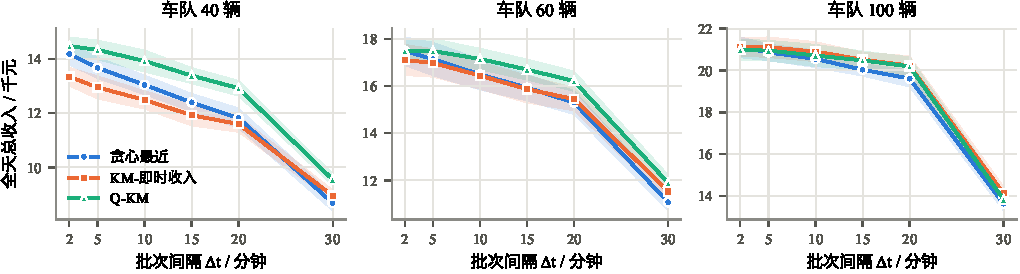
\includegraphics[width=\textwidth]{fig/exp1_revenue_dt.pdf}
	\caption{不同批次间隔 $\Dt$ 下三种策略的全天收入（10 个测试日均值，阴影为 95\% 置信区间）}
	\label{fig:exp1}
\end{figure*}

\begin{table}[t]
	\centering
	\caption{Q-KM 相对 KM 即时收入 / 最近贪心的收入增益（\%）}
	\label{tab:exp1gain}
	\small
	\setlength{\tabcolsep}{3.2pt}
	\begin{tabular}{c rr rr rr}
		\toprule
		& \multicolumn{2}{c}{40 辆} & \multicolumn{2}{c}{60 辆} & \multicolumn{2}{c}{100 辆} \\
		\cmidrule(lr){2-3}\cmidrule(lr){4-5}\cmidrule(lr){6-7}
		$\Dt$/min & vs KM & vs 贪心 & vs KM & vs 贪心 & vs KM & vs 贪心 \\
		\midrule
		\tabinput{tables/exp1_gain.tex}
		\bottomrule
	\end{tabular}
\end{table}

\begin{table}[t]
	\centering
	\caption{$\Dt=10$ min、60 辆车时的详细指标（10 个测试日均值；收入后为 95\% 置信区间半宽）}
	\label{tab:exp1detail}
	\small
	\setlength{\tabcolsep}{2.6pt}
	\resizebox{\columnwidth}{!}{\begin{tabular}{lccccc}
		\toprule
		策略 & 收入/元 & 送客/km & 应答率/\% & 接驾/km & 响应/min \\
		\midrule
		\tabinput{tables/exp1_detail.tex}
		\bottomrule
	\end{tabular}}
\end{table}

\Cref{fig:exp1} 和\cref{tab:exp1gain} 给出了 18 种设置下的结果，可以归纳出以下几点。

\textbf{(1) 运力越紧张，长期价值越重要。} 40 辆车时，Q-KM 相对 KM 即时收入在各 $\Dt$ 下增收 6.7\%–12.4\%，60 辆车时增收 2.4\%–5.4\%，均显著。100 辆车时，Q-KM 与 KM 的差距在 $\pm$2.1\% 以内，6 种设置中只有 2 种显著，而且都是 Q-KM 略低。此时验证集选出的 $\beta$ 均落在最小档 0.2–0.4，说明运力充足时到处都有空车，区域价值差异提供的信息很少。

\textbf{(2) KM 即时收入在运力紧张时不如最近贪心。} 40 辆、$\Dt=10$ 时，KM 即时收入为 \num{12494} 元，最近贪心为 \num{13050} 元。只看本批次车费的匹配偏向长途单，长途单把司机带离热点区域，空车又不会自行返回。Q-KM 的边权中包含 $\gamma V(t{+}1,i)$ 一项，代表“司机留在原地”的机会成本，这一缺陷由此得到修正（\cref{tab:exp1detail}：应答率从 59.0\% 升至 65.4\%）。

\textbf{(3) 批次间隔的影响。} 三种策略的收入都随 $\Dt$ 增大而单调下降，从 $\Dt=20$ 到 $\Dt=30$ 骤降 23\%–31\%。原因是订单耐心只有 20 分钟，比批次间隔还短，大量订单在下一批次执行前就已取消。另一方面，$\Dt$ 增大时 Q-KM 相对最近贪心的优势也在扩大（40 辆时从 2.1\% 升到 10.1\%）：批次越大，候选匹配越多，价值引导的选择余地也越大。$\Dt=2$–5 分钟时收入最高，平均响应时间（等待 + 接驾）也最短，是三者之间较好的折中。

\begin{figure*}[t]
	\centering
	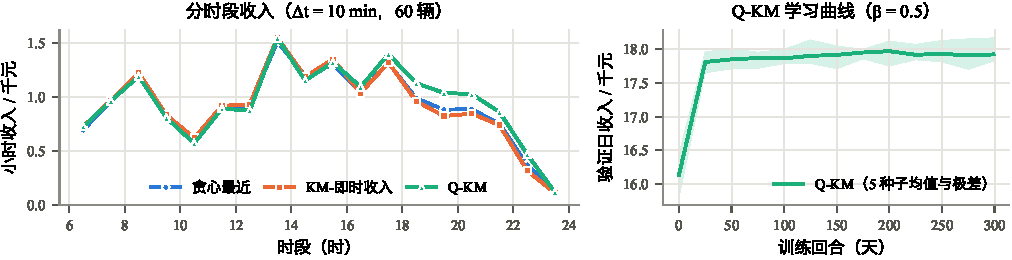
\includegraphics[width=\textwidth]{fig/exp1_hourly_curve.pdf}
	\caption{左：$\Dt=10$ min、60 辆车时按小时分解的收入；右：Q-KM 在验证日上的学习曲线（5 个种子）}
	\label{fig:hourly}
\end{figure*}

\textbf{(4) 收入从何而来。} 按小时分解（\cref{fig:hourly} 左）后可以看到，Q-KM 在 7:00–15:00 的收入反而比 KM 低 0.2\%–8.1\%：它会拒绝把司机派往冷区的高价订单，宁可让司机留在原地。到了 16:00 之后，Q-KM 的收入持续领先，18:00–22:00 时段高出 16\%–47\%。也就是说，Q-KM 的增益是\textbf{跨时段的}：白天保持车辆的空间分布，换来晚高峰更多的可用运力。批次级的贪心与 KM 只看当前批次，无法做出这种跨时段的取舍。学习曲线显示，训练约 25 个模拟日后验证收入即趋于稳定，最终验证收入在 5 个种子之间的极差约为 1.9\%。

\subsection{实验二：双目标帕累托前沿}

本节与拓展 A 共用同一组批次：8:00、13:00、18:00、23:00 各随机抽取 5 个批次，每批 40 个司机、80 个订单，距离量化到 10\,m。每个批次先用 \cref{sec:exact} 的方法求出精确前沿 $Z^\ast$，作为真值。三种进化算法各运行 5 个种子，加权和 KM 是确定性方法，只运行一次。所有指标都以 $Z^\ast$ 的理想点和最差点归一化：HV 比为 $\mathrm{HV}/\mathrm{HV}^\ast$，IGD 与 IGD$^+$ 越小越好，“命中率”指近似解中恰好落在 $Z^\ast$ 上的比例。

\begin{figure}[t]
	\centering
	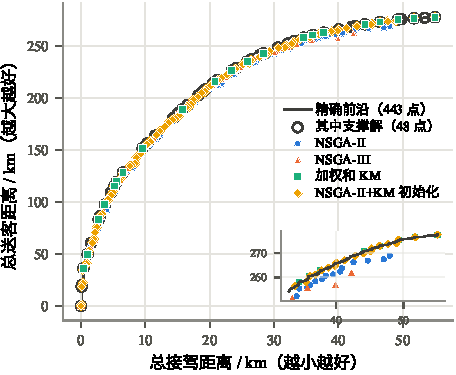
\includegraphics[width=\columnwidth]{fig/exp2_front.pdf}
	\caption{18:00 代表批次的帕累托前沿（右下为高收入端放大）。空心圆为精确前沿上的支撑解}
	\label{fig:front}
\end{figure}

\textbf{前沿形状与折中解。} \Cref{fig:front} 中，前沿在低接驾端很陡、在高收入端很平，边际收益递减明显。以与两端点连线距离最远的点（膝点）为折中方案，20 个批次平均只需最大接驾距离的 31.6\%，就能获得最大送客距离的 71.1\%。这说明平台若完全追求收入最大化，最后约 29\% 的收入需要付出约 68\% 的额外接驾距离。

\begin{table}[t]
	\centering
	\caption{近似算法对比（20 批次 × 5 种子均值；末列为以 IGD$^+$ 计的 Friedman 平均秩）}
	\label{tab:moo}
	\resizebox{\columnwidth}{!}{%
	\begin{tabular}{lccccccc}
		\toprule
		方法 & HV 比$\uparrow$ & IGD$\downarrow$ & IGD$^+\downarrow$ & Spacing$\downarrow$ & 解数 & 命中率/\% & 秩 \\
		\midrule
		\tabinput{tables/exp24_methods.tex}
		\bottomrule
	\end{tabular}}
\end{table}

\begin{figure}[t]
	\centering
	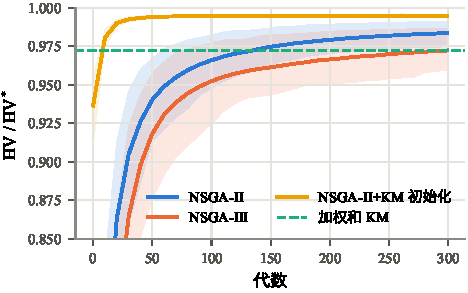
\includegraphics[width=\columnwidth]{fig/exp2_convergence.pdf}
	\caption{HV 比随代数的收敛（100 条曲线的均值，阴影为 10\%–90\% 分位）}
	\label{fig:conv}
\end{figure}

\textbf{算法比较。} 由\cref{tab:moo} 和\cref{fig:conv} 可以得到三点结论。(1) 两个目标时，NSGA-II 明显优于 NSGA-III：HV 比为 0.984 对 0.972，Spacing 为 0.47 对 0.84。NSGA-III 的参考方向在归一化目标空间中按角度均匀分布，而本问题的前沿弯曲程度很大，解会集中在少数方向上，拥挤距离反而能更好地适应局部密度。(2) 加权和 KM 每次都解到真正的最优，命中率达 98.9\%（未命中的点来自 $\lambda=0$ 时只最大化收入、接驾距离不唯一的弱支配解）。但它平均只找到 21.4 个点，HV 比仅 0.972，IGD$^+$ 是各方法中最差的。(3) KM 初始化把加权和 KM 的精确解作为“锚点”，NSGA-II 在锚点之间继续搜索非支撑解。这一做法使 HV 比提高到 0.995，IGD$^+$ 从 0.0071 降到 0.0033（约 54\%），命中率从 31\% 升到 55\%，并且在第 20 代左右就超过随机初始化 300 代的水平。

\textbf{统计检验。} 以 20 个批次为区组、IGD$^+$ 为指标做 Friedman 检验，$p=2.9\times10^{-11}$。四种方法的平均秩依次为 KM 初始化 1.0、NSGA-II 2.1、NSGA-III 3.2、加权和 3.7。Nemenyi 临界差 CD $=1.05$（$\alpha=0.05$），因此前三者两两之间差异显著，NSGA-III 与加权和之间不显著。配对 Wilcoxon 检验得到相同结论：KM 初始化对 NSGA-II，以及 NSGA-II 对加权和，均有 $p<10^{-5}$。

\subsection{拓展实验 A：精确前沿揭示的结构}

\begin{figure}[t]
	\centering
	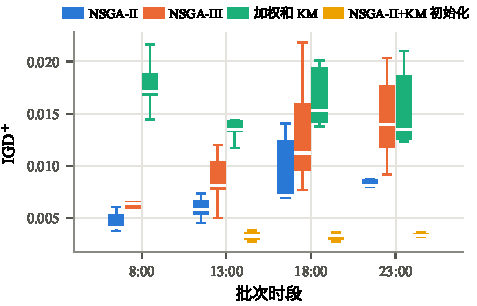
\includegraphics[width=\columnwidth]{fig/exp4_igd_hour.pdf}
	\caption{不同时段批次上各方法的 IGD$^+$（越小越好；每箱 5 个批次，每批取 5 个种子均值）}
	\label{fig:igdhour}
\end{figure}

20 个批次的精确前沿全部通过了 \cref{sec:exact} 中的逐点验证，修复次数为 0。每个批次平均有 445 个非支配点（306–593 个），平均需要求解 1335 次整数规划，点数最多的批次（593 点）在单进程下约需 3.4 分钟。主要发现如下：

\textbf{(1) 帕累托前沿以非支撑解为主。} 位于下凸包上的支撑解平均只有 43.5 个，占 \textbf{10.0\%}（各批次在 8.0\%–14.4\% 之间）。任何线性加权方法，无论 $\lambda$ 取得多密，都只能覆盖这约 10\% 的点。离散匹配问题的可行组合非常多，相邻的支撑解之间分布着大量“凹陷处”的折中解，这正是进化算法相对加权和方法的优势所在。此前的作业只把 HV 比作为评价依据，加权和 KM 与 NSGA-II 的 HV 比只差约 0.01，看起来接近。有了精确前沿，可以确认两者的差距真实存在，主要体现在前沿的覆盖率上（IGD$^+$ 相差 2.2 倍）。

\textbf{(2) 难度随时段变化。} \Cref{fig:igdhour} 中，18:00 和 23:00 批次的可行订单更多（平均 63 和 71 单，8:00 与 13:00 均约 59 单），前沿点更多，随机初始化的 NSGA-II/III 误差明显增大。KM 初始化在四个时段上的 IGD$^+$ 都稳定在 0.003 左右，对问题规模不敏感。

\textbf{(3) 对作业中“竞争比”的补充。} 若以精确前沿为基准，NSGA-II 找到的最高送客距离平均为 269.3\,km，比真实最大值 278.5\,km 低 3.3\%；而 KM 初始化与加权和 KM 都能达到真实最大值。可见随机初始化的进化算法在前沿两端收敛不足，用精确解作锚点可以弥补这一点。


\subsection{拓展实验 B：DV-KM 深度价值网络}

\begin{figure*}[t]
	\centering
	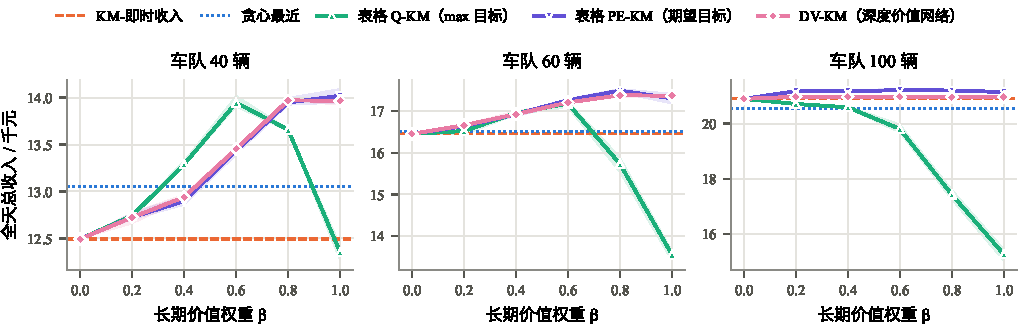
\includegraphics[width=\textwidth]{fig/exp3_beta.pdf}
	\caption{长期价值权重 $\beta$ 对全天收入的影响（$\Dt=10$ min，10 个测试日；阴影为 3 个训练种子的极差）}
	\label{fig:beta}
\end{figure*}

\begin{table*}[t]
	\centering
	\caption{各方法收入（元）。“最佳”列为测试集上的最佳 $\beta$（括号内，仅作上界参考），“$\beta=1$”列为 3 个种子的均值 $\pm$ 标准差}
	\label{tab:dvkm}
	\small
	\setlength{\tabcolsep}{6pt}
	{\begin{tabular}{l cc cc cc}
		\toprule
		& \multicolumn{2}{c}{40 辆} & \multicolumn{2}{c}{60 辆} & \multicolumn{2}{c}{100 辆} \\
		\cmidrule(lr){2-3}\cmidrule(lr){4-5}\cmidrule(lr){6-7}
		方法 & 最佳 & $\beta{=}1$ & 最佳 & $\beta{=}1$ & 最佳 & $\beta{=}1$ \\
		\midrule
		\tabinput{tables/exp3_main.tex}
		\bottomrule
	\end{tabular}}
\end{table*}

\Cref{fig:beta} 和\cref{tab:dvkm} 比较了三种价值估计方式，表格 PE-KM 用于分解两个因素的作用。

\textbf{max 目标是 $\beta$ 增大后收入崩溃的主因。} 表格 Q-KM 的收入在 $\beta=0.6$ 附近达到峰值，随后迅速下降。$\beta=1$ 时，60 辆和 100 辆车的收入分别只有 \num{13560} 元和 \num{15252} 元，比 KM 即时收入低 17.6\% 和 27.0\%，应答率从 0.79 跌到 0.63（100 辆）。同样是表格结构，把 TD 目标改成期望型的 PE-KM 后，收入随 $\beta$ 增大基本单调上升或保持平稳，$\beta=1$ 时为 \num{17302} 元和 \num{21145} 元。由此可以判断，崩溃来自 max 自举的过估计，而不是区域离散化。被高估的“原地等待”价值使大量正收益的边权变成负值，KM 便选择不派。拓展 D 将进一步说明，起作用的并不是高估的幅度，而是高估在“等待”与“出发”之间的不对称。

\textbf{深度网络带来鲁棒性，但没有带来更高的收入峰值。} DV-KM 在 3 个车队规模、6 个 $\beta$ 取值下都没有出现崩溃，$\beta=1$ 时种子间的标准差最小（23–56 元）。但它的最佳收入与表格 PE-KM 基本持平（40 辆 \num{13970} 对 \num{14019}，60 辆 \num{17376} 对 \num{17487}），100 辆时还低约 1.1\%。原因在于，本仿真中订单量与区域划分的比例使 $8\times8$ 表格的每个状态都有充足的样本，连续坐标的精细度没有可利用的空间。可以预期，在更细的空间粒度或样本更稀疏的城市中，函数逼近的泛化能力才会体现为收入优势。

\begin{table}[t]
	\centering
	\caption{DV-KM 消融（60 辆，同一份 175 万条经验，收入/元）}
	\label{tab:ablation}
	\small
	\setlength{\tabcolsep}{2.2pt}
	\begin{tabular}{lccccc}
		\toprule
		变体 \textbackslash\ $\beta$ & 0.2 & 0.4 & 0.6 & 0.8 & 1.0 \\
		\midrule
		\tabinput{tables/exp3_ablation.tex}
		\bottomrule
	\end{tabular}
\end{table}

\textbf{平滑正则是网络稳定的关键。} \Cref{tab:ablation} 中，用相同数据重新训练（仅随机初始化不同）引起的波动约 1.2\%；去掉粗编码后收入下降不超过 0.7\%，与这一波动处于同一量级。去掉平滑正则后，收入在 $\beta=0.4$ 时达到全表最高的 \num{17585} 元，但 $\beta\ge0.8$ 时跌回 \num{15744}/\num{14794} 元，与表格 Q-KM 的崩溃形态相同。缺少空间平滑时，网络在样本稀疏的位置会外推出虚高的价值，作用与 max 偏差类似。这与 CVNet\cite{tang2019deep}强调 Lipschitz 约束的动机一致。

\begin{figure*}[t]
	\centering
	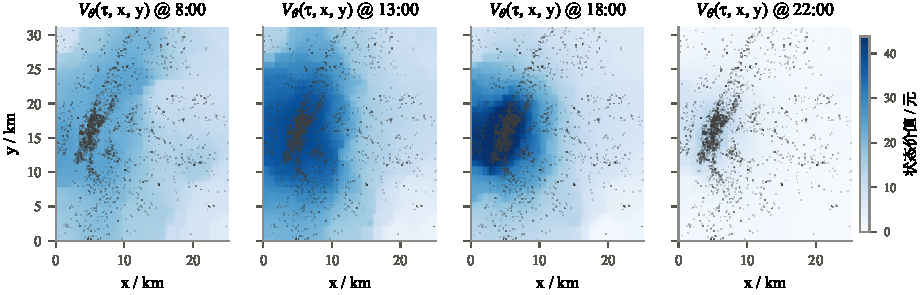
\includegraphics[width=0.92\textwidth]{fig/exp3_vmap.pdf}
	\caption{DV-KM 学到的连续价值函数 $V_\theta(\tau,x,y)$（60 辆车，灰点为训练期签到点）}
	\label{fig:vmap}
\end{figure*}

\Cref{fig:vmap} 展示了学到的价值面：13:00–18:00 曼哈顿中城与下城（$x\approx5$–10\,km，$y\approx12$–20\,km）的价值最高；8:00 时价值分布较分散，高值区尚未集中；22:00 整体价值趋近于 0，因为营业即将结束，剩余可赚的时间很短。价值面在空间上连续平滑，没有表格方法在网格边界处的阶跃。

\subsection{拓展实验 C：离事后最优还有多远}

\begin{table*}[t]
	\centering
	\caption{事后最优区间与在线策略（5 个测试日均值，与实验一配对）。“KM”“Q-KM”列为收入占 LB 的百分比；“弥合”为 Q-KM 弥合的 (LB$-$KM) 缺口比例。$^\dagger$：该设置有 4 天 MILP 在 400\,s 内未收敛，只报 UB，比例以 UB 为分母（是达成率的下界）}
	\label{tab:hindsight}
	\small
	\setlength{\tabcolsep}{5pt}
	{\begin{tabular}{c cccc cccc cccc}
		\toprule
		& \multicolumn{4}{c}{40 辆} & \multicolumn{4}{c}{60 辆} & \multicolumn{4}{c}{100 辆} \\
		\cmidrule(lr){2-5}\cmidrule(lr){6-9}\cmidrule(lr){10-13}
		$\Dt$ & [LB, UB]/千元 & KM & Q-KM & 弥合 & [LB, UB]/千元 & KM & Q-KM & 弥合 & [LB, UB]/千元 & KM & Q-KM & 弥合 \\
		\midrule
		\tabinput{tables/exp5.tex}
		\bottomrule
	\end{tabular}}
\end{table*}

\Cref{tab:hindsight} 给出了 \cref{sec:hindsight} 的事后最优区间。LB 是一个可执行的事后计划，因而真实的事后最优不低于 LB；表中以 LB 为分母的达成率因此是\textbf{偏乐观的}，在线策略离最优的实际差距只会更大。除 100 辆、$\Dt=10$ 外，所有 LB 都由 MILP 求到最优，回放仿真器后收入与 LB 逐日一致。

\textbf{运力紧张、批次较密时，短视的代价最大。} $\Dt=10$ 时，即使只用接驾按最坏情况计的保守计划，事后也能拿到 \num{17416} 元（40 辆）和 \num{20602} 元（60 辆）。KM 即时收入只达到其中的 71\% 和 81\%，Q-KM 达到 81\% 和 85\%，即 Q-KM 弥合了 KM 与事后最优之间 33\% 和 18\% 的缺口。这说明 Q-KM 的长期价值确实把策略推向了离线最优的方向，但仍有至少 15\%–19\% 的收入因不知道未来而损失；若以 UB 计，Q-KM 只达到 73\%/79\%。100 辆车时 KM 已达到 UB 的 87\%，Q-KM 没有额外收益，与实验一中“运力充足时长期价值无用”的结论一致。

\textbf{大批次间隔下的损失主要是结构性的。} $\Dt$ 从 10 增大到 30 分钟，事后最优本身就下降约三分之一（40 辆的 LB 从 \num{17416} 降至 \num{11407} 元，60 辆从 \num{20602} 降至 \num{13425} 元）。此时上下界只相差 4\%–5\%，在线策略的达成率反而升高到 80\%–93\%。也就是说，实验一中 $\Dt=30$ 时的收入骤降，大部分是“订单在下一批次前就已取消”造成的，即便事先知道全部订单也无法挽回，并不是派单算法的失误。批次间隔这一\textbf{系统设计参数}，比在给定间隔下改进匹配算法更重要。


\subsection{拓展实验 D：崩溃的根源是“等待被高估”}

\begin{figure*}[t]
	\centering
	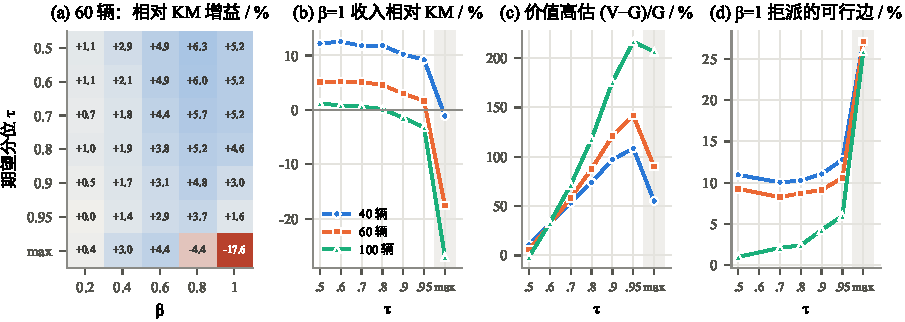
\includegraphics[width=\textwidth]{fig/exp6_expectile.pdf}
	\caption{价值目标乐观度谱（$\Dt=10$ min，3 个训练种子 × 10 个测试日）。(a) 60 辆车时各 $(\tau,\beta)$ 相对 KM 即时收入的增益；(b) $\beta=1$ 时的收入；(c) 价值表相对真实折扣回报的高估（$\beta=0.6$ 策略）；(d) $\beta=1$ 派单时边权 $\le0$、被拒派的可行边比例。灰色区域为 max 目标}
	\label{fig:expectile}
\end{figure*}

\begin{table}[t]
	\centering
	\caption{$\beta=1$ 时可行边上的平均价值项（元，3 种子 × 5 测试日）}
	\label{tab:gostay}
	\small
	\setlength{\tabcolsep}{3pt}
	\begin{tabular}{llcccc}
		\toprule
		车队 & 目标 & 出发 & 等待 & 出发$-$等待 & 出发/等待 \\
		\midrule
		\tabinput{tables/exp6b.tex}
		\bottomrule
	\end{tabular}
\end{table}

拓展 B 把 Q-KM 的崩溃归因于 max 目标的过估计。如果这一解释成立，那么任何足够乐观的目标都应当同样崩溃。\Cref{fig:expectile} 用期望分位目标检验了这个推论，结果与之相反。

\textbf{高估的幅度不能解释崩溃。} 随着 $\tau$ 增大，价值表的高估单调上升（\cref{fig:expectile}(c)）。$\tau=0.95$ 时高估达到 109\%/142\%/217\%（40/60/100 辆），与 max 目标的 55\%/90\%/206\% 相当，甚至更高。但 $\tau=0.95$ 在 $\beta=1$ 时的收入仍为 KM 的 $+9.2$\%/$+1.6$\%/$-3.2$\%，而 max 目标是 $-1.1$\%/$-17.6$\%/$-27.0$\%（\cref{fig:expectile}(b)）。在各自最佳的 $\beta$ 下，$\tau$ 从 0.5 增大到 0.95 只让增益平滑地下降 1.2–2.5 个百分点，热力图上也看不到 max 目标在右下角出现的断崖（\cref{fig:expectile}(a)）。

\textbf{决定性的是高估落在哪里。} \Cref{tab:gostay} 把边权中的长期项拆成“出发”$\gamma^{\Delta}V(t{+}\Delta,k)$ 与“等待”$\gamma V(t{+}1,i)$。期望分位目标把两者近似同比例放大：$\tau$ 从 0.5 到 0.95，出发/等待之比始终在 0.88–0.93 之间，因而在边权的差分中大部分相互抵消。max 目标则不同：与 $\tau=0.95$ 相比，它的出发价值低 5.8–10.9 元，等待价值只低 0.1–7.0 元，出发/等待之比降到 0.84，长期项从 PE 的 $-2.3$ 至 $-6.4$ 元扩大到 $-11.7$ 至 $-12.3$ 元。结果有 26\%–27\% 的可行边被判为负权而不派（\cref{fig:expectile}(d)），而期望分位目标下这一比例不超过 13\%。

\textbf{一个解释：max 的乐观按决策时点累积。} Q-learning 的目标在每个决策时点对 $\mathcal{A}(s')\cup\{\text{等待}\}$ 取一次 max，等于假设司机下一时刻总能接到附近最好的订单。原地等待的司机每 10 分钟就经历一个决策时点，送客的司机在 $\Delta$ 个时间片里只在到达时经历一次。因此单位时间内，等待状态积累的乐观远多于出发状态，平台被系统性地诱导去“等更好的单”。期望分位的乐观则作用在每次更新所采样的回报上，等待转移的回报几乎是确定的（无收入、仍在原区域），不会因决策时点多而额外放大。这一解释与\cref{tab:gostay} 中“max 只压低出发/等待之比”的现象一致，但严格验证还需要控制决策频率的对照实验。这一结论说明，改进长期价值派单的关键不在于压低价值的整体水平，而在于保证不同动作之间的\textbf{相对}价值无偏。


\subsection{拓展实验 E：批次级权衡在全天是否成立}

\begin{figure*}[t]
	\centering
	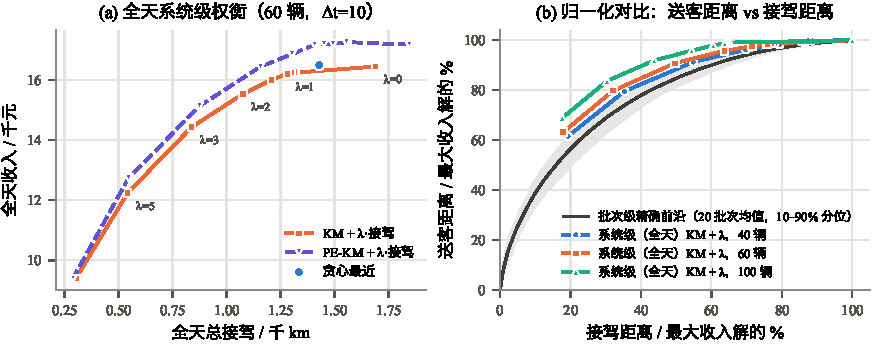
\includegraphics[width=\textwidth]{fig/exp7_system_front.pdf}
	\caption{(a) 在 KM / PE-KM 边权中加入接驾惩罚 $\lambda\cdot2p_{dj}$ 后的全天收入–总接驾距离（10 个测试日均值）；(b) 以最大收入解为 100\% 归一化后，批次级精确前沿与全天系统级曲线的对比}
	\label{fig:system}
\end{figure*}

实验二与拓展 A 都在单个批次内讨论“收入–接驾”的权衡。但平台真正关心的是全天累计的指标，单批次的前沿是否反映系统层面的代价，需要另行检验。为此在全天仿真中把边权改为 $w_{dj}=\text{fare}_j-\lambda\cdot2p_{dj}$（$\lambda=1$ 表示 1\,km 接驾与 1\,km 送客等价），扫描 $\lambda\in[0,8]$，分别作用于 KM 即时收入和表格 PE-KM（$\beta=0.6$），$\Dt\in\{5,10,20\}$，三种车队。

\textbf{全天层面的权衡远比单批次平缓。} \Cref{fig:system}(b) 中，三条全天曲线都位于批次级精确前沿的上方。在单个批次内，把接驾距离压缩 20\% 平均要损失 3.0\% 的送客距离，压缩 35\% 要损失 7.7\%。在全天层面，KM 只需取 $\lambda=0.25$，接驾总距离就下降 12\%/22\%/35\%（40/60/100 辆），而收入只变化 $-0.0$\%/$-1.2$\%/$-1.1$\%。换成 PE-KM，同一 $\lambda$ 下接驾下降 11\%–25\%，收入反而上升 0.1\%–0.5\%；40 辆车、$\lambda=0.5$ 时收入上升 1.0\%。$\Dt=5$ 与 20 分钟时结论相同：在全部 12 种（$\Dt$，车队，基础策略）组合下，$\lambda=0.25$ 使接驾下降 8\%–35\%，收入变化在 $-1.2$\% 至 $+0.5$\% 之间。直到 $\lambda\ge2$，即接驾惩罚开始切断大量正收益的边，收入才明显下降（$\lambda=2$ 时 $-4$\% 至 $-6$\%，$\lambda=3$ 时 $-10$\% 至 $-13$\%）。

\textbf{原因是批次之间的替代与运力回收。} 单批次前沿假设“这一批没派的订单就丢了”。但订单耐心（20 分钟）不短于批次间隔，被远处司机放弃的订单往往在本批次由近处司机接走，或在下一批次被其他司机服务，批次级的收入损失大部分在后续批次中被收回。另一方面，接驾时间本身占用运力：缩短接驾使司机更早空闲，在运力紧张时直接转化为更多的服务单量。这与网约车经济学中“空驶追单”（wild goose chase）的论断一致\cite{castillo2017surge}。最近贪心在 60/100 辆时接驾距离比 KM 短 15\%/34\%，收入差距却在 $\pm$1.7\% 以内，也印证了这一点。

由此得出一个实际的结论：以批次级帕累托前沿上的代价来权衡乘客体验和平台收入，会把真实代价\textbf{高估数倍}。在本仿真中，存在一段近乎“免费”的区间（$\lambda\approx0.25$–1），可以显著缩短接驾而几乎不损失收入。多目标派单应在系统层面评估，而不仅仅在单个批次上求前沿。


\section{结论与局限}

本报告在纽约签到驱动的派单仿真上完成了收入对比、帕累托前沿和两项拓展实验，结论如下。(1) 长期价值的作用取决于运力是否紧张。Q-KM 在 40/60 辆车、各批次间隔下显著优于 KM 即时收入与最近贪心，增收来自“白天保持空间分布、晚高峰兑现运力”这一跨时段取舍；100 辆车时不再有优势。批次间隔一旦超过订单耐心，收入会骤降。(2) 派单的双目标前沿以非支撑解为主，加权和方法在原理上只能覆盖前沿的一小部分。以精确前沿为真值，NSGA-II 优于 NSGA-III；用 KM 解初始化种群后，近似质量进一步提高，并且统计显著。(3) Q-KM 在大 $\beta$ 下的失效主要来自 max 自举的过估计，期望型的策略评估目标可以消除这一问题。深度价值网络提供了对 $\beta$ 的鲁棒性和连续的价值面，前提是加入空间平滑正则，但在本数据规模下没有带来更高的收入峰值。进一步的乐观度谱实验表明，崩溃并不取决于高估的幅度，而取决于高估在“等待”与“出发”之间是否对称；长期价值派单需要的是动作间相对价值无偏。(4) \HINDSIGHTCONC (5) 单批次前沿会把收入–接驾的权衡代价高估数倍：由于批次间的订单替代和运力回收，较小的接驾惩罚几乎不损失全天收入，多目标派单应在系统层面评估。

\textbf{局限。} 订单由签到数据构造，与真实打车需求存在偏差；仿真中空闲司机不会主动调度；价值函数与精确前沿都只针对单个批次或单一城市。今后可以把价值网络与空车调度联合优化，并把 Q-KM 的长期价值边权作为第三个目标，在全天层面研究“收入–接驾距离–应答率”的系统级前沿。

\begin{thebibliography}{99}
\small
\setlength{\itemsep}{0pt}
\bibitem{xu2018large} Xu Z, Li Z, Guan Q, et al. Large-scale order dispatch in on-demand ride-hailing platforms: A learning and planning approach[C]//Proceedings of the 24th ACM SIGKDD International Conference on Knowledge Discovery \& Data Mining. 2018: 905--913.
\bibitem{tang2019deep} Tang X, Qin Z, Zhang F, et al. A deep value-network based approach for multi-driver order dispatching[C]//Proceedings of the 25th ACM SIGKDD International Conference on Knowledge Discovery \& Data Mining. 2019: 1780--1790.
\bibitem{deb2002fast} Deb K, Pratap A, Agarwal S, et al. A fast and elitist multiobjective genetic algorithm: NSGA-II[J]. IEEE Transactions on Evolutionary Computation, 2002, 6(2): 182--197.
\bibitem{deb2014evolutionary} Deb K, Jain H. An evolutionary many-objective optimization algorithm using reference-point-based nondominated sorting approach, part I: Solving problems with box constraints[J]. IEEE Transactions on Evolutionary Computation, 2014, 18(4): 577--601.
\bibitem{kuhn1955hungarian} Kuhn H W. The Hungarian method for the assignment problem[J]. Naval Research Logistics Quarterly, 1955, 2(1--2): 83--97.
\bibitem{tong2016online} Tong Y, She J, Ding B, et al. Online mobile micro-task allocation in spatial crowdsourcing[C]//2016 IEEE 32nd International Conference on Data Engineering (ICDE). 2016: 49--60.
\bibitem{watkins1992q} Watkins C J C H, Dayan P. Q-learning[J]. Machine Learning, 1992, 8(3): 279--292.
\bibitem{hasselt2010double} van Hasselt H. Double Q-learning[C]//Advances in Neural Information Processing Systems 23. 2010: 2613--2621.
\bibitem{haimes1971bicriterion} Haimes Y Y, Lasdon L S, Wismer D A. On a bicriterion formulation of the problems of integrated system identification and system optimization[J]. IEEE Transactions on Systems, Man, and Cybernetics, 1971, SMC-1(3): 296--297.
\bibitem{mavrotas2009effective} Mavrotas G. Effective implementation of the $\varepsilon$-constraint method in multi-objective mathematical programming problems[J]. Applied Mathematics and Computation, 2009, 213(2): 455--465.
\bibitem{zitzler1999multiobjective} Zitzler E, Thiele L. Multiobjective evolutionary algorithms: A comparative case study and the strength Pareto approach[J]. IEEE Transactions on Evolutionary Computation, 1999, 3(4): 257--271.
\bibitem{ishibuchi2015modified} Ishibuchi H, Masuda H, Tanigaki Y, et al. Modified distance calculation in generational distance and inverted generational distance[C]//Evolutionary Multi-Criterion Optimization (EMO 2015). Springer, 2015: 110--125.
\bibitem{demsar2006statistical} Dem\v{s}ar J. Statistical comparisons of classifiers over multiple data sets[J]. Journal of Machine Learning Research, 2006, 7: 1--30.
\bibitem{huangfu2018parallelizing} Huangfu Q, Hall J A J. Parallelizing the dual revised simplex method[J]. Mathematical Programming Computation, 2018, 10(1): 119--142.
\bibitem{yang2015modeling} Yang D, Zhang D, Zheng V W, et al. Modeling user activity preference by leveraging user spatial temporal characteristics in LBSNs[J]. IEEE Transactions on Systems, Man, and Cybernetics: Systems, 2015, 45(1): 129--142.
\bibitem{kostrikov2022offline} Kostrikov I, Nair A, Levine S. Offline reinforcement learning with implicit Q-learning[C]//International Conference on Learning Representations (ICLR). 2022.
\bibitem{newey1987asymmetric} Newey W K, Powell J L. Asymmetric least squares estimation and testing[J]. Econometrica, 1987, 55(4): 819--847.
\bibitem{bunte2009overview} Bunte S, Kliewer N. An overview on vehicle scheduling models[J]. Public Transport, 2009, 1(4): 299--317.
\bibitem{castillo2017surge} Castillo J C, Knoepfle D, Weyl G. Surge pricing solves the wild goose chase[C]//Proceedings of the 2017 ACM Conference on Economics and Computation (EC). 2017: 241--242.
\end{thebibliography}
\end{document}
